\documentclass{article}
\usepackage[UTF8]{ctex}
\usepackage{pythonhighlight}
\usepackage{markdown}
\usepackage{listings}
\lstset{
    basicstyle          =   \tt,          % 基本代码风格
    identifierstyle=\color{brown!80!black},
    keywordstyle        =   \color{purple}\bfseries,          % 关键字风格
    commentstyle        =   \rmfamily\itshape,  % 注释的风格,斜体
    stringstyle         =   \ttfamily,  % 字符串风格
    flexiblecolumns,                % 别问为什么,加上这个
    numbers             =   left,   % 行号的位置在左边
    showspaces          =   false,  % 是否显示空格,显示了有点乱,所以不现实了
    numberstyle         =   \zihao{-5}\ttfamily,    % 行号的样式,小五号,tt等宽字体
    showstringspaces    =   false,
    captionpos          =   t,      % 这段代码的名字所呈现的位置,t指的是top上面
    frame               =   lrtb,   % 显示边框
    backgroundcolor=\color[RGB]{245,245,244},
}


% Language setting
% Replace `english' with e.g. `spanish' to change the document language
\usepackage[english]{babel}
\usepackage{float}
% Set page size and margins
% Replace `letterpaper' with `a4paper' for UK/EU standard size
\usepackage[letterpaper,top=2cm,bottom=2cm,left=3cm,right=3cm,marginparwidth=1.75cm]{geometry}

% Useful packages
\usepackage{amsmath}
\usepackage{graphicx}
\usepackage[colorlinks=true, allcolors=blue]{hyperref}

\title{普物虚拟实验报告4}
\author{雷远航 \ 学号:3210105807}

\begin{document}

\maketitle

\begin{abstract}
    光栅分光仪测波长
\end{abstract}

\section*{一、实验目的}
\subsection*{- 训练分光计的调整与使用技巧}
\subsection*{- 了解光栅衍射原理}
\subsection*{- 光栅常数和入射波长的测量}


\section*{二、实验原理}
\subsection*{分光计的结构:}
\begin{figure}[H]
	\centering
	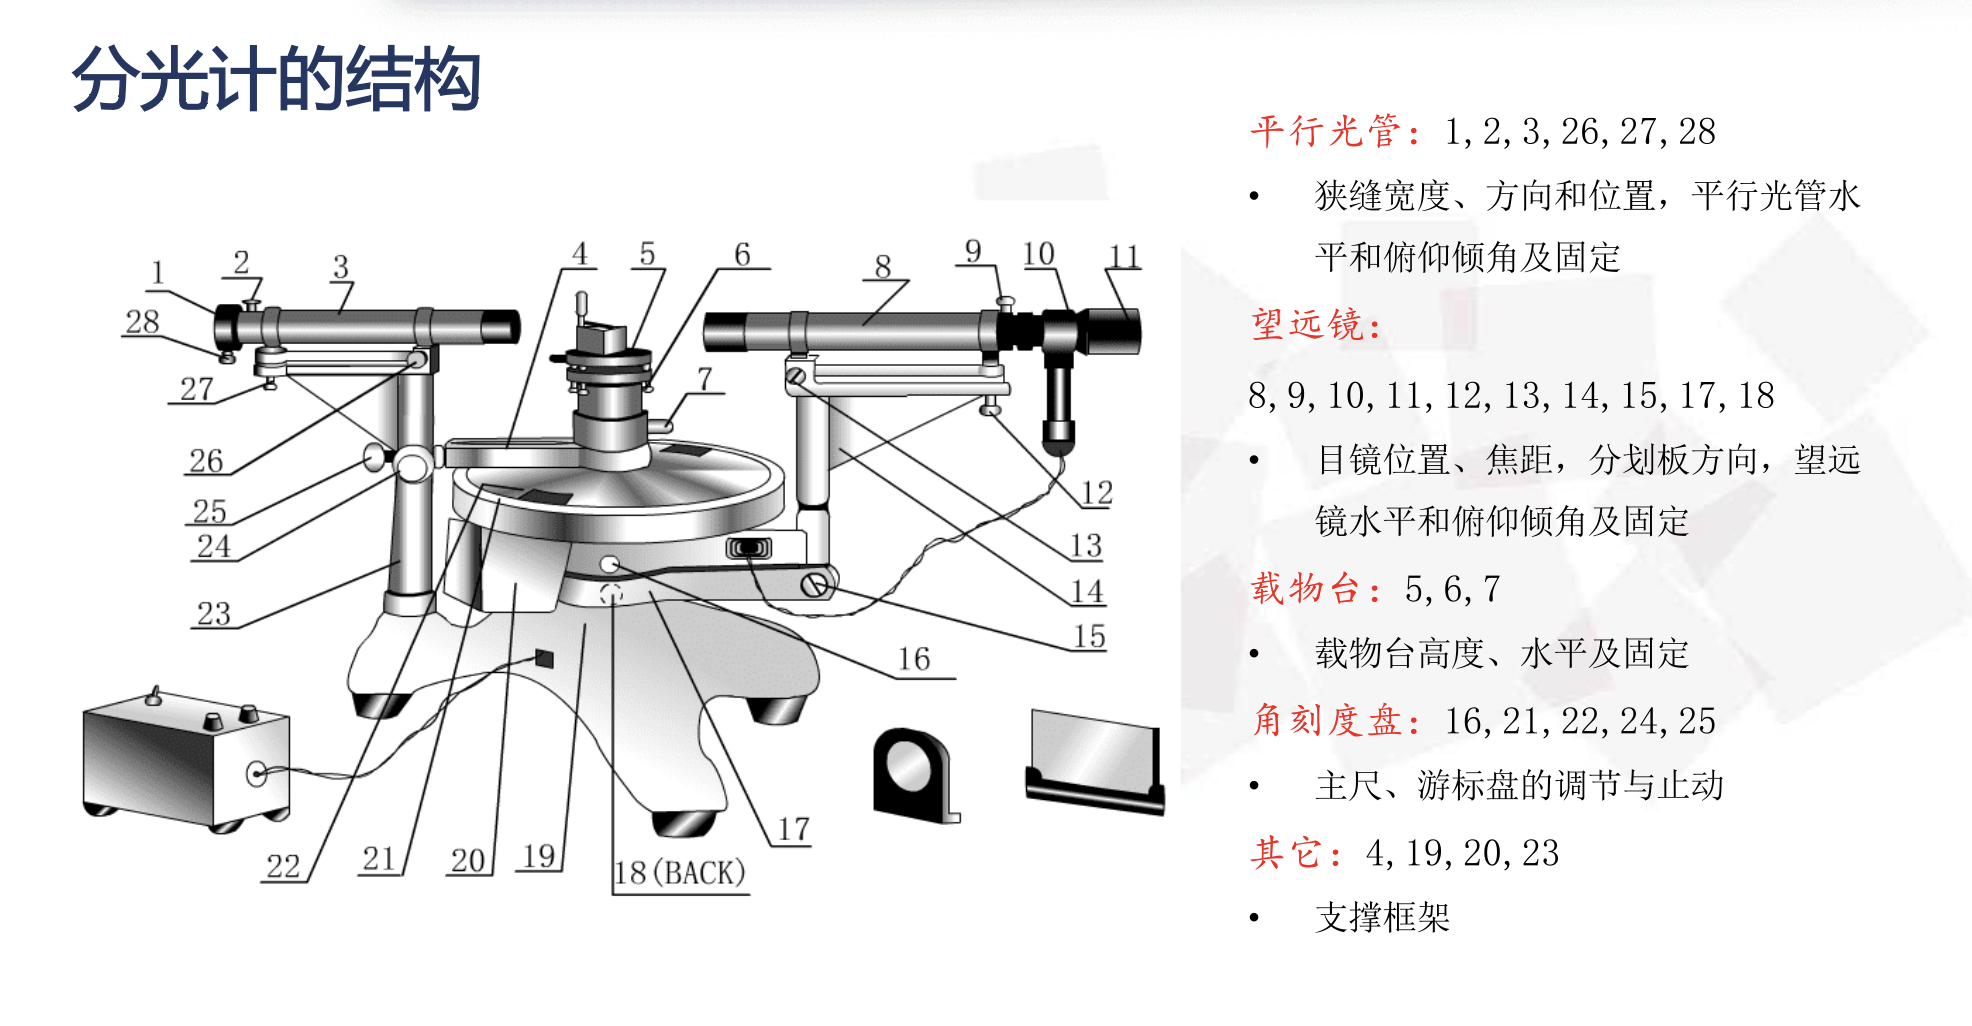
\includegraphics[width=1\textwidth]{1.png}
	\end{figure}

\subsection*{分光计的原理:}
\begin{figure}[H]
	\centering
	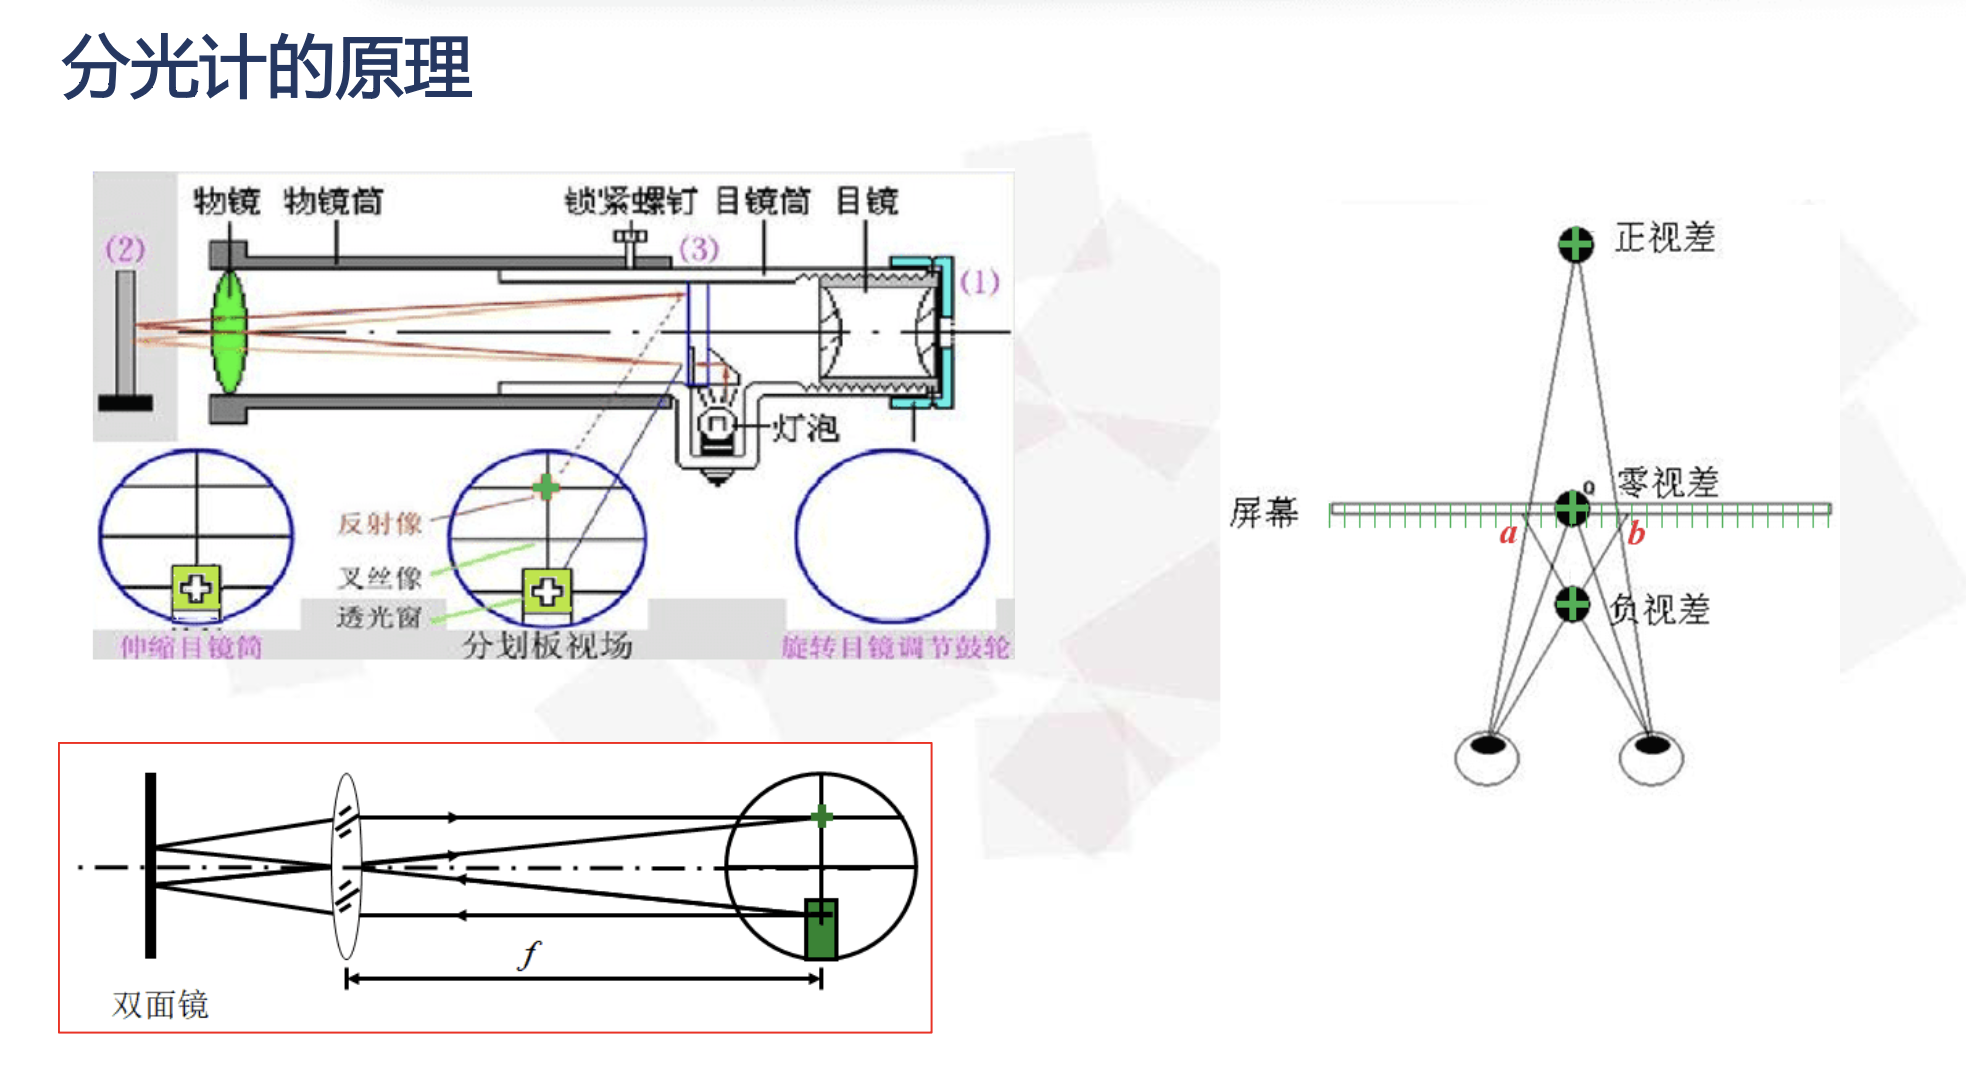
\includegraphics[width=1\textwidth]{2.png}
	\end{figure}

\subsection*{单缝夫琅和费衍射:}
\begin{figure}[H]
	\centering
	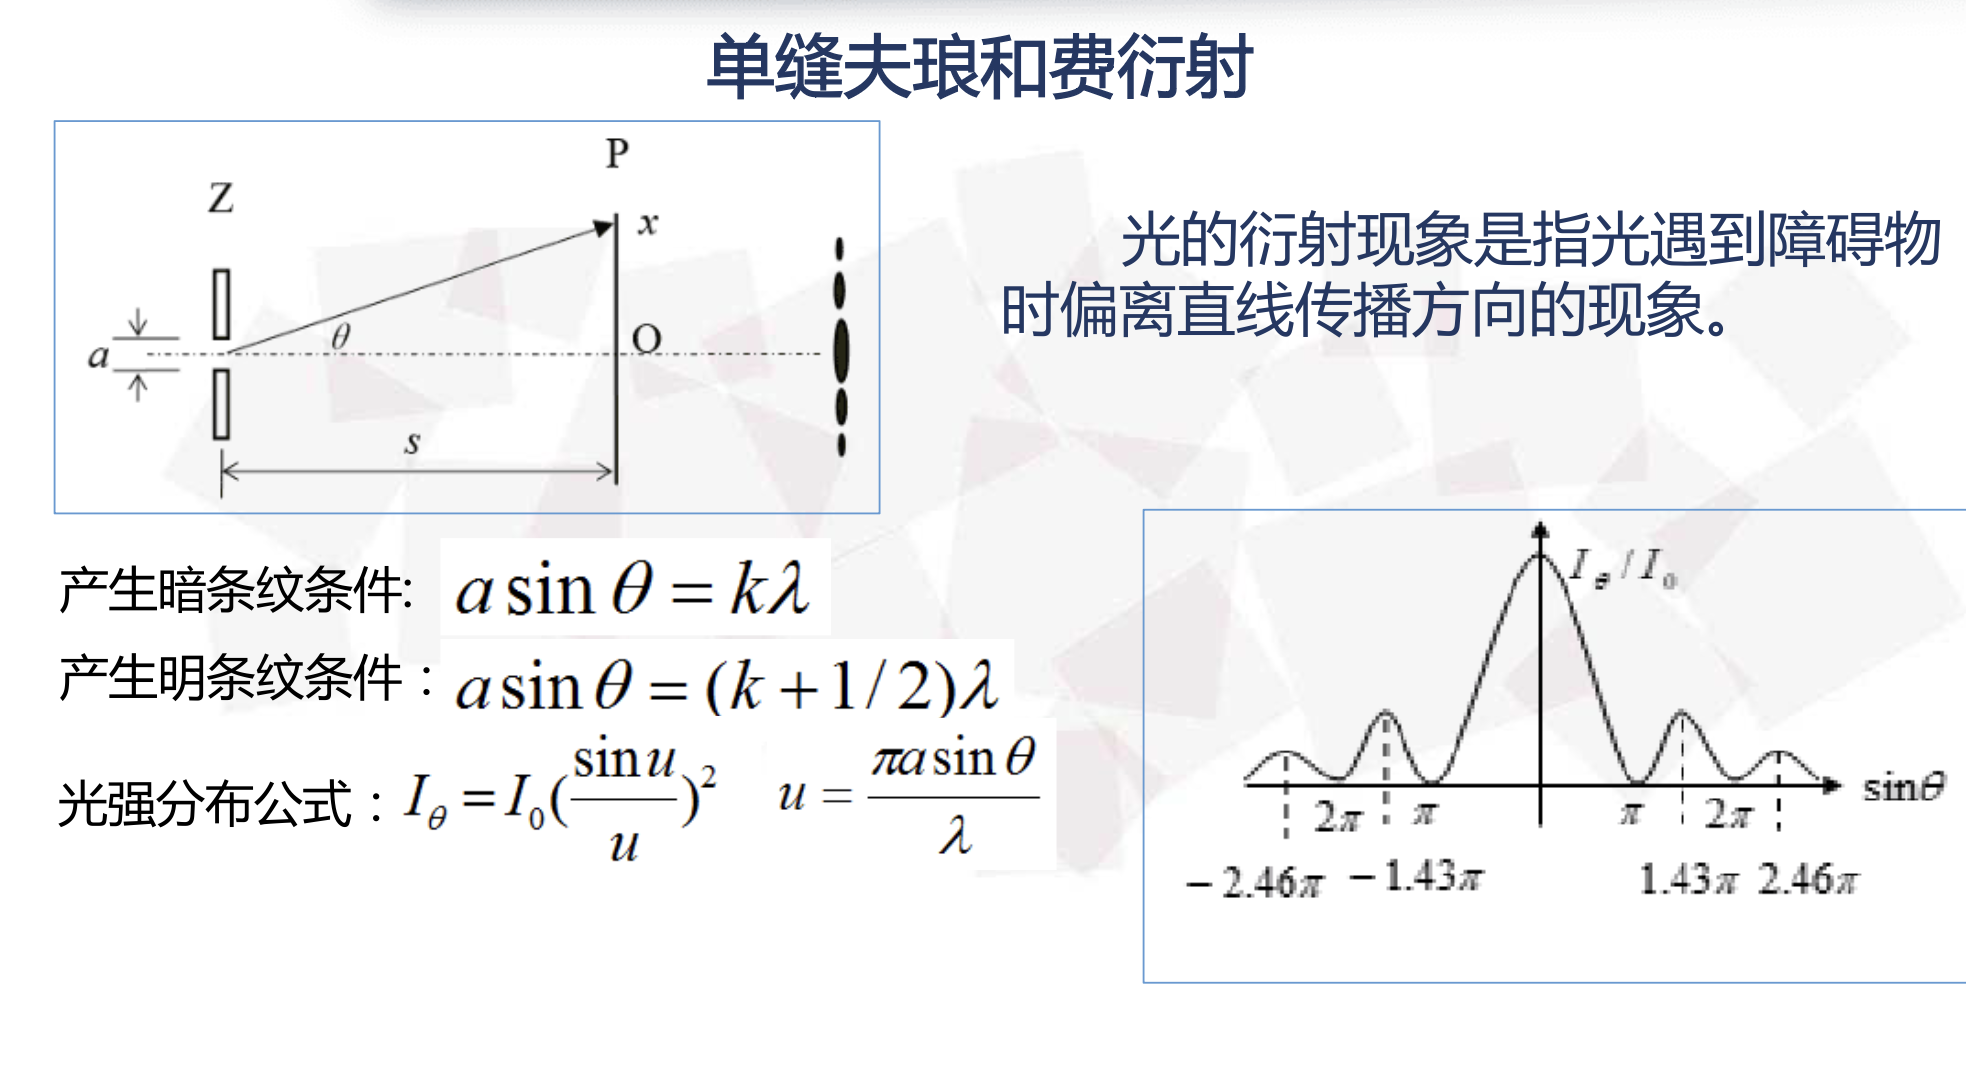
\includegraphics[width=1\textwidth]{3.png}
	\end{figure}

\subsection*{光栅衍射:}
\begin{figure}[H]
	\centering
	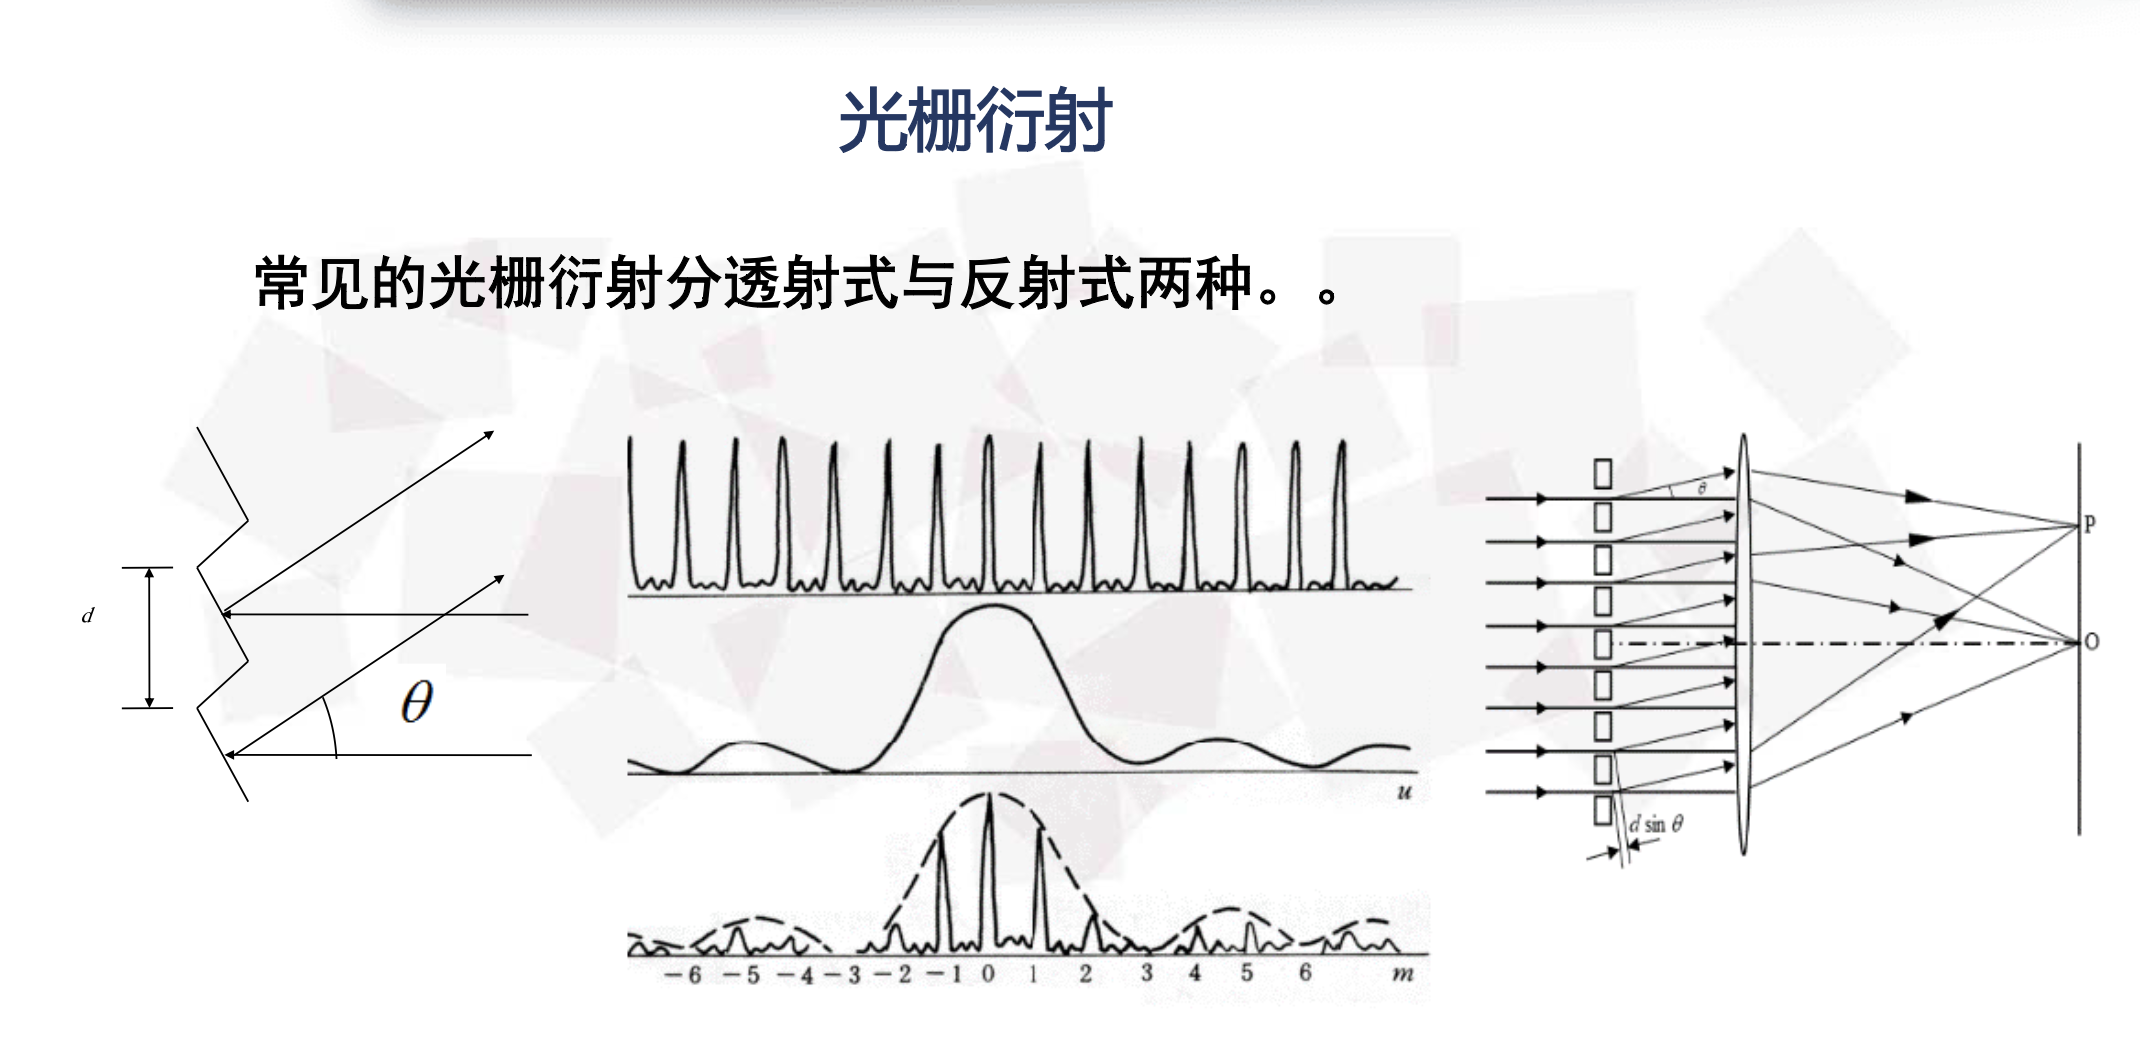
\includegraphics[width=1\textwidth]{4.png}
	\end{figure}

    \begin{figure}[H]
        \centering
        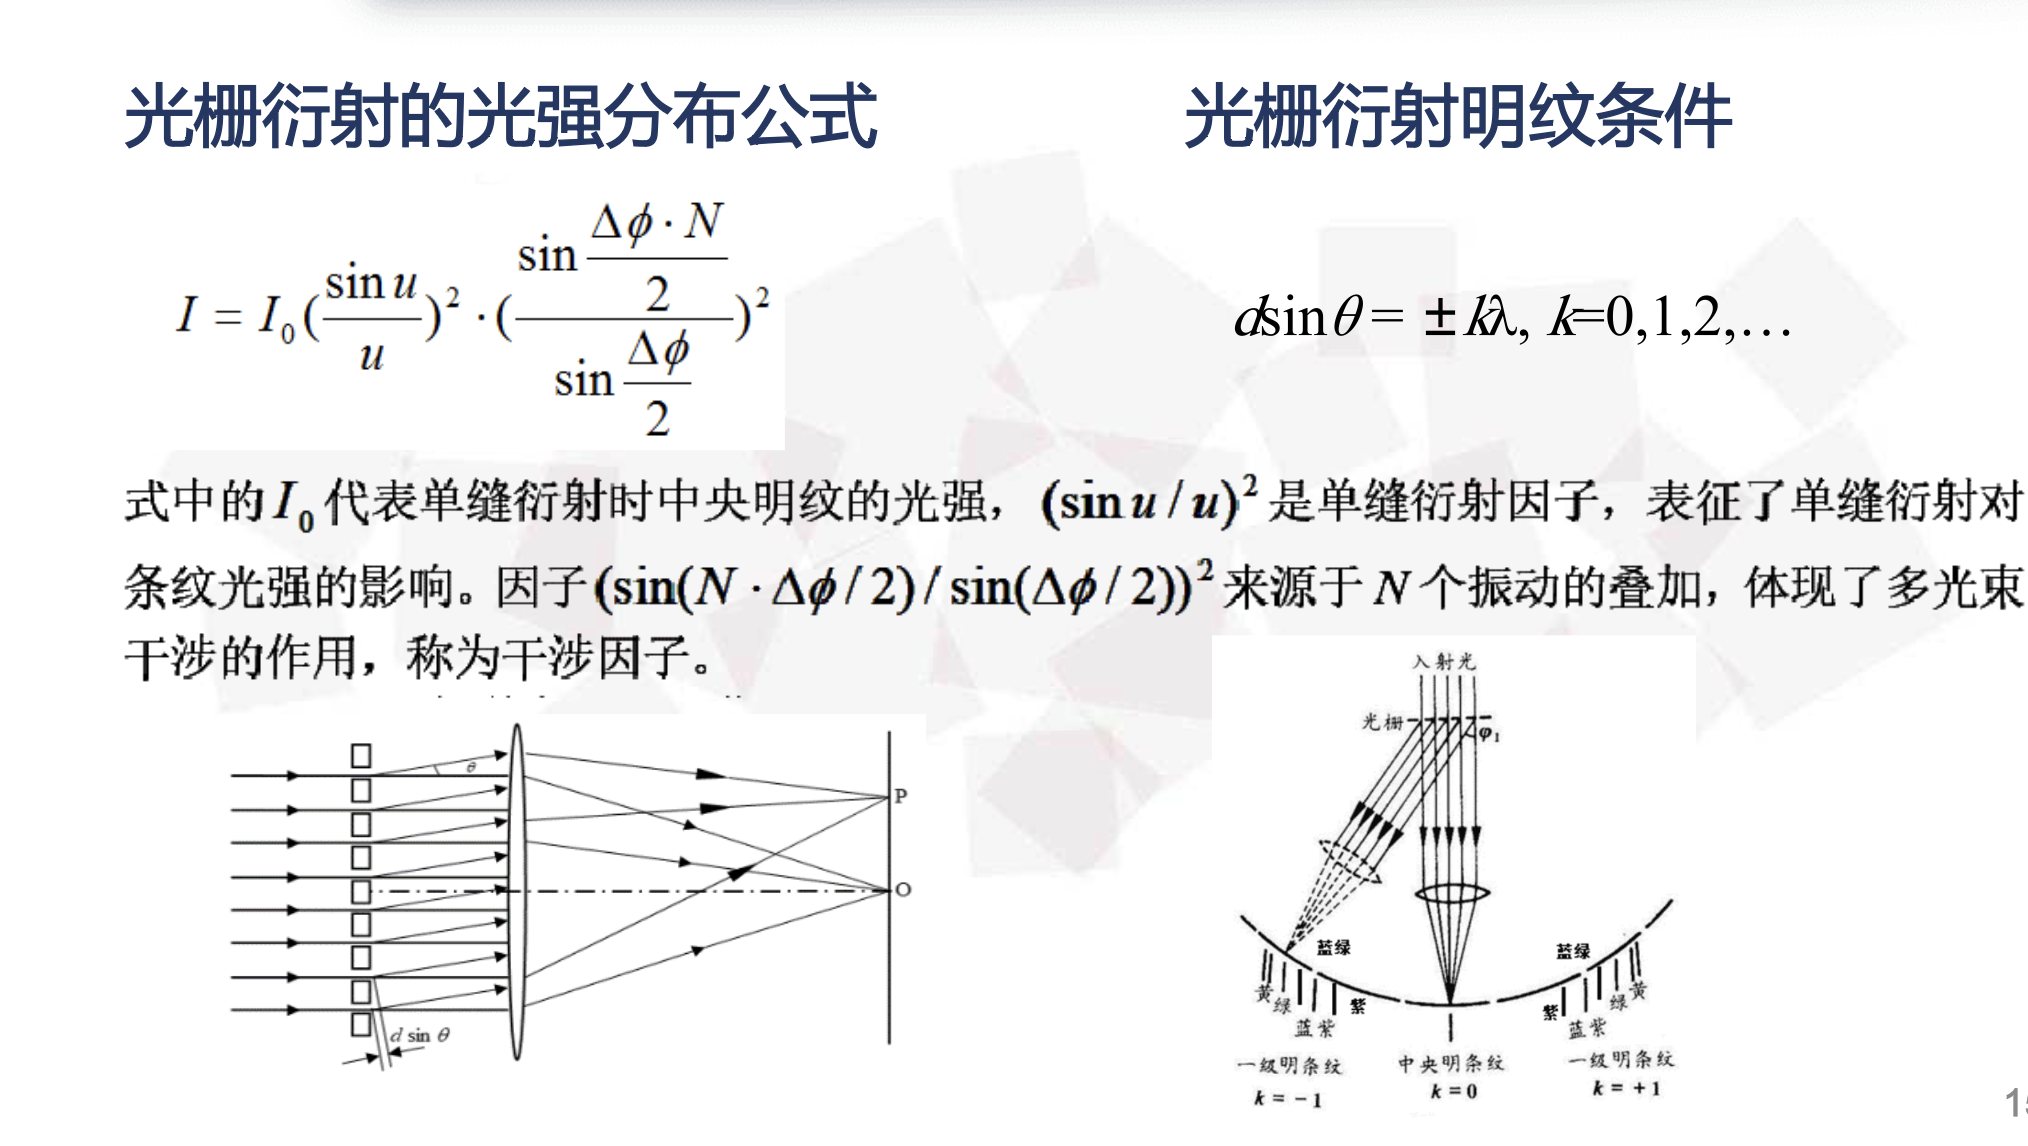
\includegraphics[width=1\textwidth]{5.png}
        \end{figure}


\section*{三、实验内容}
\subsection*{- 调节分光计}
\subsection*{- 测光栅常数与波长}
已知波长(蓝紫光491nm),测量一级与二级明纹位置,计算光栅常数;已知光栅常数,
测量明纹位置,测量波长(紫光,黄内光,黄外光)
( 6次测量,计算不确定度)

\section*{四、实验数据}

\subsection*{1.调节分光计}
在虚拟实验室中调节分光计平衡,在调平望远镜和载物台后,对目镜进行截图如下.
\begin{figure}[H]
    \centering
    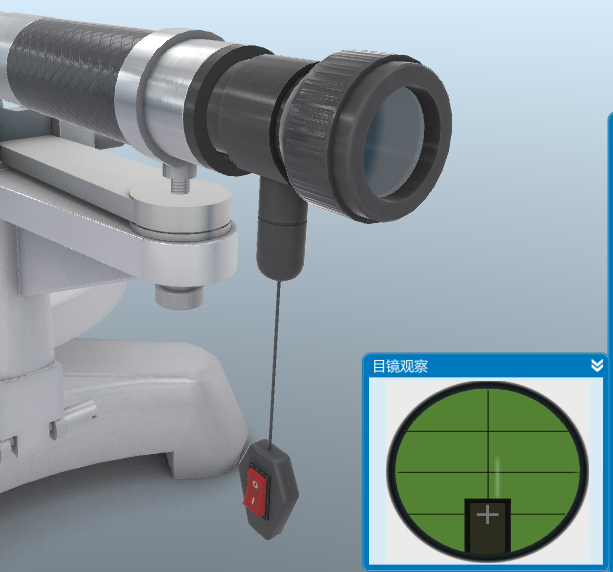
\includegraphics[width=0.5\textwidth]{23.png}
    \end{figure}

    \begin{figure}[H]
        \centering
        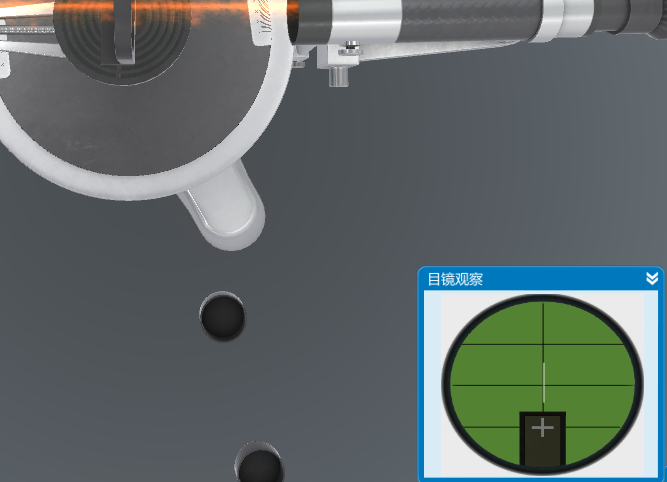
\includegraphics[width=0.5\textwidth]{24.png}
        \end{figure}
       
\subsection*{2.计算光栅常数}

\subsubsection*{实验过程中的操作记录截图:}

\begin{figure}[H]
    \centering
    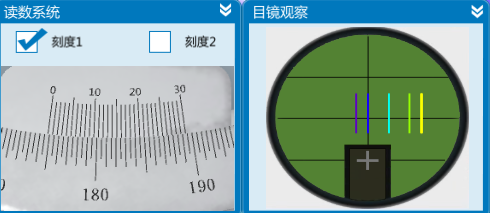
\includegraphics[width=0.5\textwidth]{11.png}
    \end{figure}

    \begin{figure}[H]
        \centering
        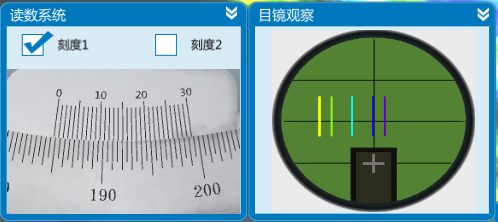
\includegraphics[width=0.5\textwidth]{12.png}
        \end{figure}
        \begin{figure}[H]
            \centering
            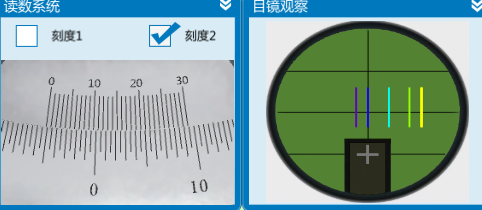
\includegraphics[width=0.5\textwidth]{13.png}
            \end{figure}

            \begin{figure}[H]
                \centering
                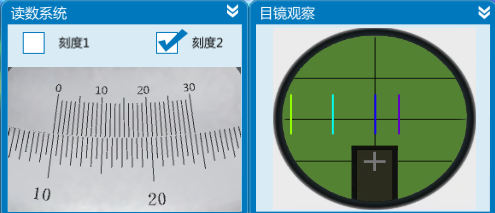
\includegraphics[width=0.5\textwidth]{14.png}
                \end{figure}

                \begin{figure}[H]
                    \centering
                    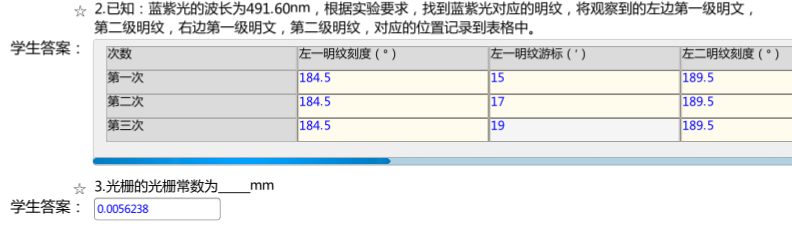
\includegraphics[width=0.5\textwidth]{31.png}
                    \end{figure}
    
\subsubsection*{处理计算数据}
\begin{figure}[H]
    \centering
    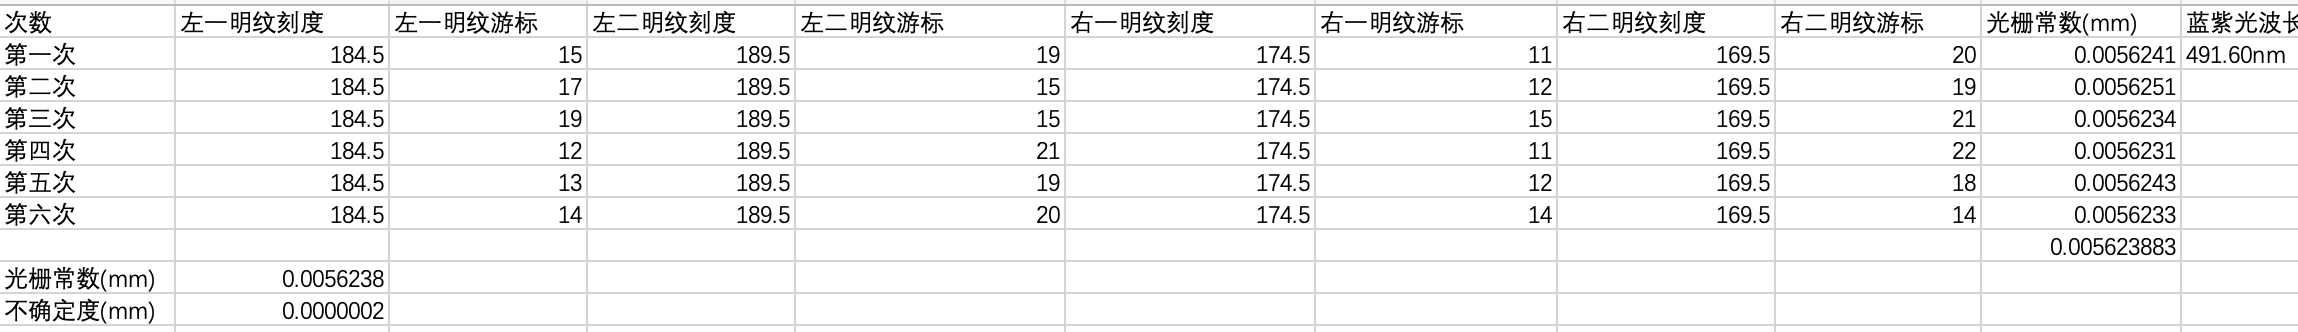
\includegraphics[width=1\textwidth]{6.png}
    \end{figure}
已知蓝紫光的波长为:491.60nm,以及光栅常数的计算公式:dsin$\theta$=k$\lambda$ 

进行六次的测量求出光栅常数的平均值与不确定度:

光栅常数(mm):0.0056238

不确定度(mm):0.0000002


\subsection*{3.计算紫光波长}
\subsubsection*{实验操作截图记录}

\begin{figure}[H]
    \centering
    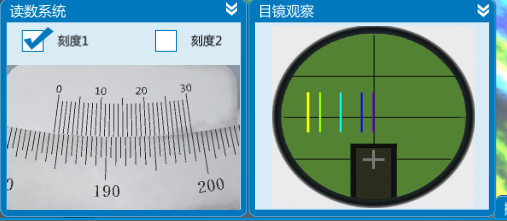
\includegraphics[width=0.5\textwidth]{15.png}
    \end{figure}

    \begin{figure}[H]
        \centering
        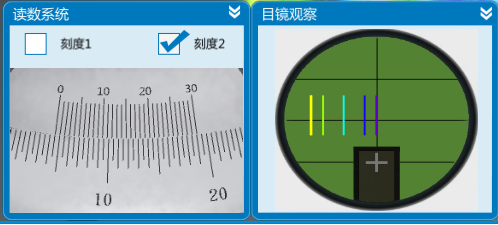
\includegraphics[width=0.5\textwidth]{16.png}
        \end{figure}
        \begin{figure}[H]
            \centering
            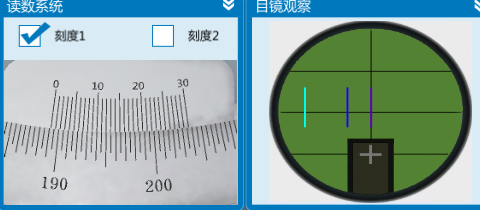
\includegraphics[width=0.5\textwidth]{17.png}
            \end{figure}

            \begin{figure}[H]
                \centering
                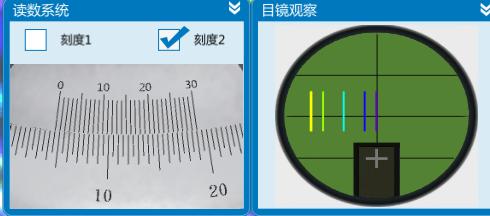
\includegraphics[width=0.5\textwidth]{18.png}
                \end{figure}
                
                \begin{figure}[H]
                    \centering
                    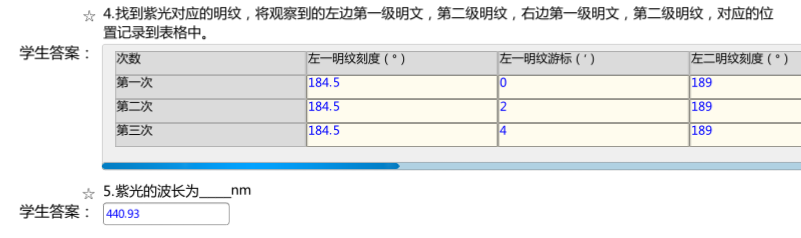
\includegraphics[width=1\textwidth]{32.png}
                    \end{figure}
    
\subsubsection*{实验数据处理计算}
\begin{figure}[H]
    \centering
    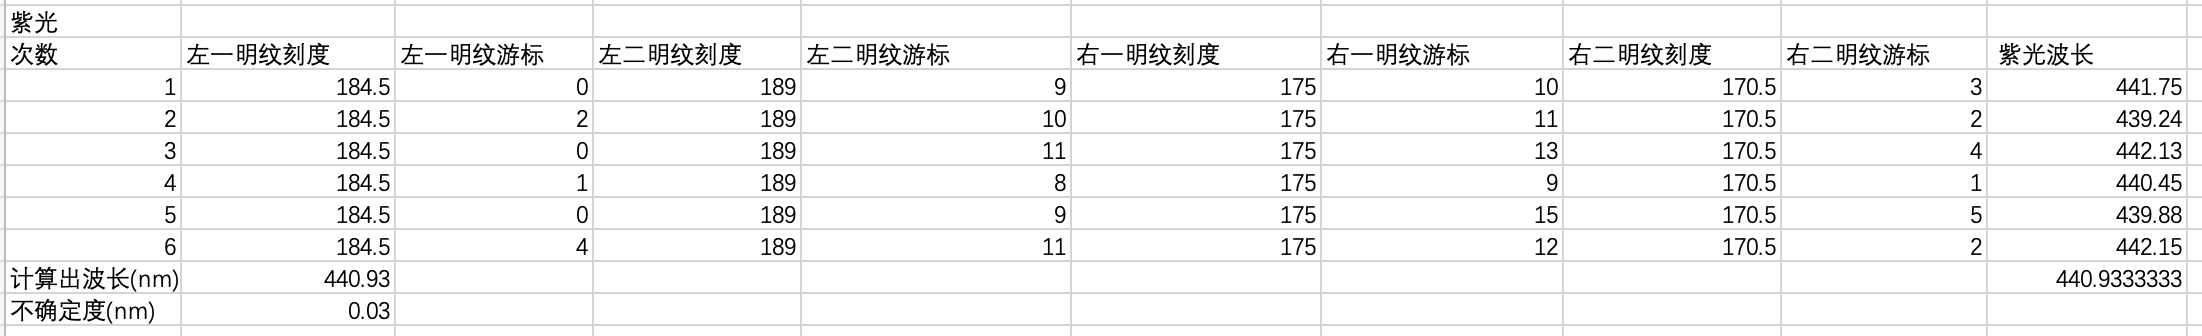
\includegraphics[width=1\textwidth]{8.png}
    \end{figure}

利用上一步中求出的光栅常数值,以及光栅公式可以求出紫光波长.

进行六次测量求出紫光波长的平均值和不确定度:

紫光波长(nm):440.93

不确定度(nm):0.03


\subsection*{4.计算黄内光波长}
\subsubsection*{实验操作记录截图}
\begin{figure}[H]
    \centering
    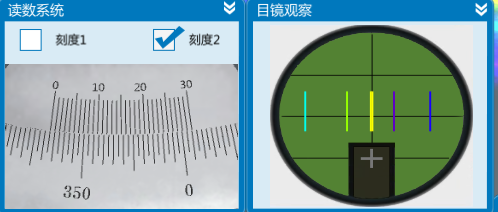
\includegraphics[width=0.5\textwidth]{19.png}
    \end{figure}

    \begin{figure}[H]
        \centering
        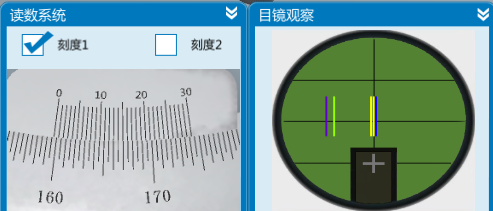
\includegraphics[width=0.5\textwidth]{20.png}
        \end{figure}
        \begin{figure}[H]
            \centering
            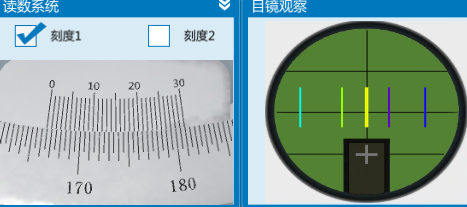
\includegraphics[width=0.5\textwidth]{21.png}
            \end{figure}

            \begin{figure}[H]
                \centering
                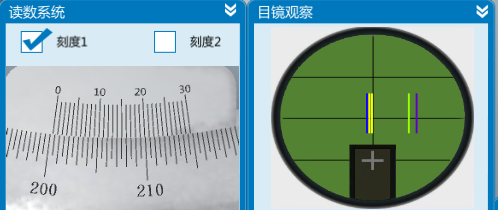
\includegraphics[width=0.5\textwidth]{22.png}
                \end{figure}
                \begin{figure}[H]
                    \centering
                    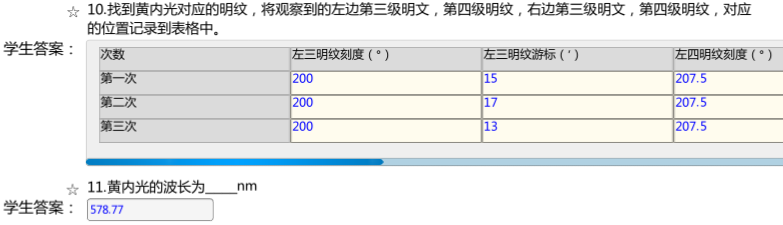
\includegraphics[width=1\textwidth]{33.png}
                    \end{figure}
    
\subsubsection*{实验数据处理计算}
\begin{figure}[H]
    \centering
    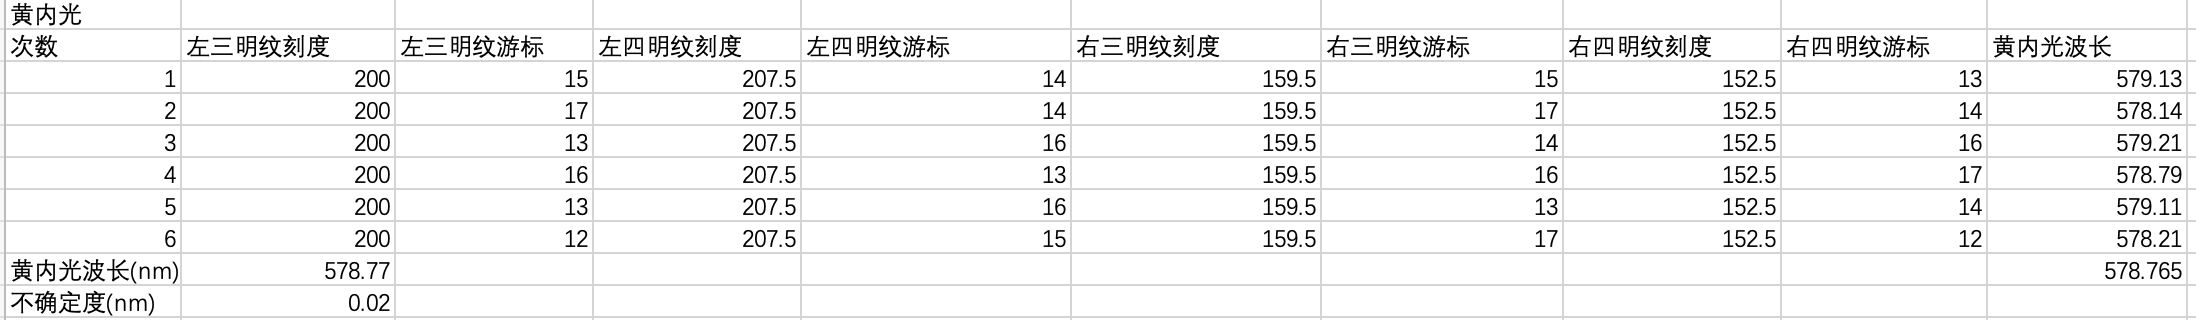
\includegraphics[width=1\textwidth]{9.png}
    \end{figure}

    利用求出的光栅常数值,以及光栅公式可以求出黄内光波长.

    进行六次测量求出黄内光波长的平均值和不确定度:
    
    紫光波长(nm):578.77
    
    不确定度(nm):0.02
    

\subsection*{5.计算黄外光波长}
\subsubsection*{实验操作记录截图}
\begin{figure}[H]
    \centering
    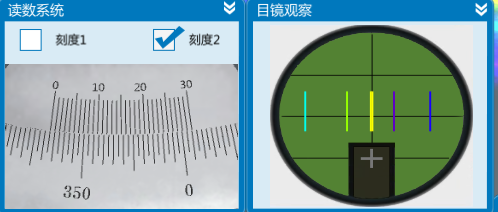
\includegraphics[width=0.5\textwidth]{19.png}
    \end{figure}

    \begin{figure}[H]
        \centering
        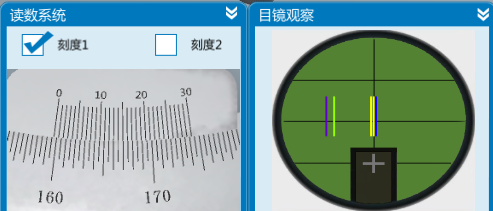
\includegraphics[width=0.5\textwidth]{20.png}
        \end{figure}
        \begin{figure}[H]
            \centering
            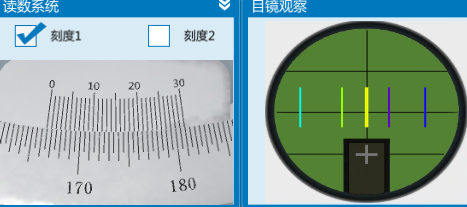
\includegraphics[width=0.5\textwidth]{21.png}
            \end{figure}

            \begin{figure}[H]
                \centering
                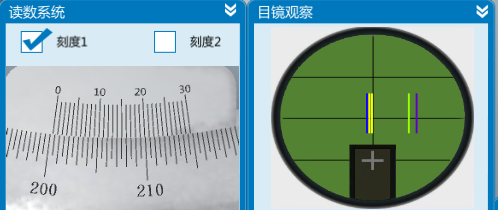
\includegraphics[width=0.5\textwidth]{22.png}
                \end{figure}
                \begin{figure}[H]
                    \centering
                    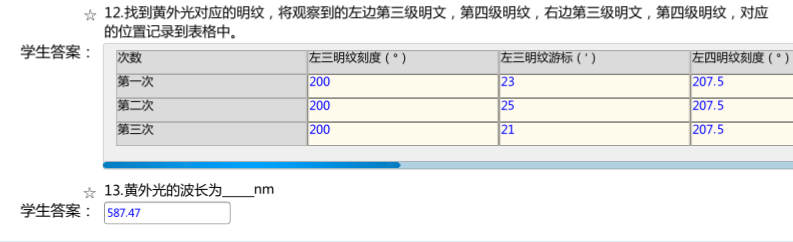
\includegraphics[width=1\textwidth]{34.png}
                    \end{figure}
    
\subsubsection*{实验数据处理计算}
\begin{figure}[H]
    \centering
    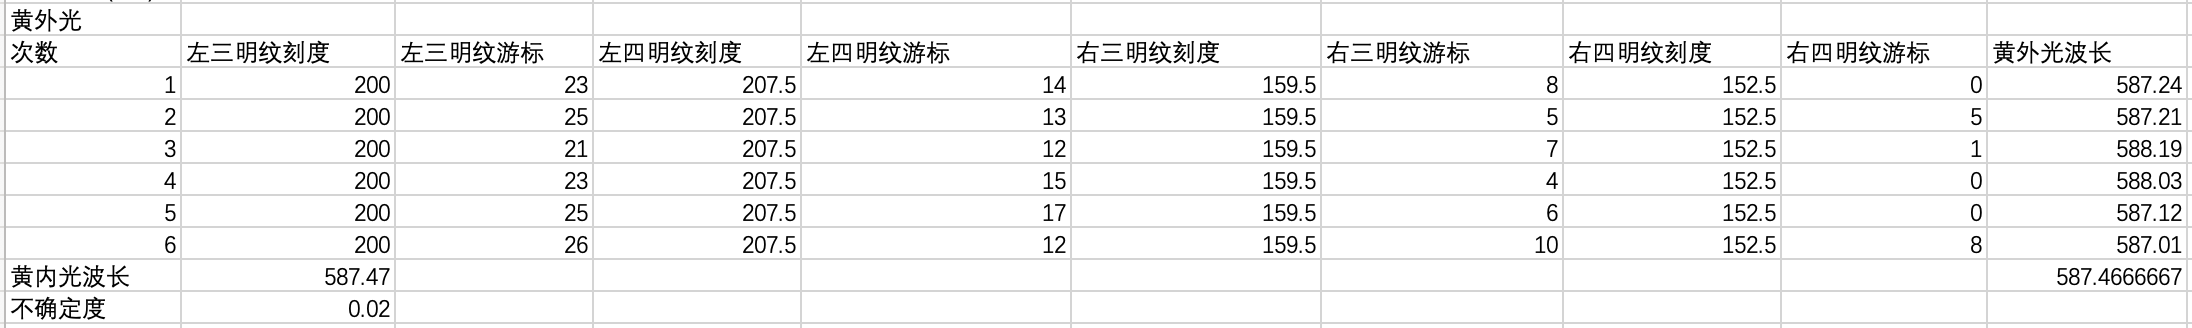
\includegraphics[width=1\textwidth]{10.png}
    \end{figure}

    利用求出的光栅常数值,以及光栅公式可以求出黄外光波长.

    进行六次测量求出黄外光波长的平均值和不确定度:
    
    紫光波长(nm):587.47
    
    不确定度(nm):0.02

     


\section*{五、分析与总结}

\subsection*{思考题}
\subsubsection*{1.调节分光计时所使用的双平面反射镜起了什么作用?能否用三棱镜
代替平面镜来调整望远镜?}

调节分光计时所使用的双平面反射镜起的作用有:

1、使望远镜对平行光聚焦

2、使望远镜光轴垂直于仪器主轴:要求望远镜光轴与分光计的主轴垂直, 以保证观察面是一个平面,以获得正确的测量结果。

不能用三棱镜,虽然经三棱镜反射光线可能平行,但光线反射回去的位置已经和原来射出位置不同,这样就无法确定垂直了。 

\subsubsection*{2.如果调节时从望远镜中观察到平面镜的两个反射像如下图所示,怎
样调节能最快的将十字叉丝像与上十字线重合?写出调节步骤。}
\begin{figure}[H]
    \centering
    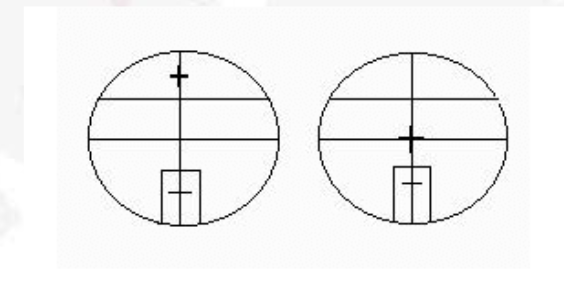
\includegraphics[width=0.5\textwidth]{25.png}
    \end{figure}


    (1)用平台螺钉把右图的十字叉丝象调上去1.5厘米,再使平台转180度, 调节望远镜俯仰螺钉使十字叉丝象与重合。
    
    (2)用平台螺钉把右图的十字叉丝象调至上十字线,再使平台转180度,(此时叉丝象在上十字线下方1厘米处),用望远镜和平台螺钉分别把十字叉丝象上调0.5厘米。

    \subsection*{实验总结}
本次的线上实验的操作难度相比于前三次线上实验难度大了很多,首先对分光计进行平衡的调节就花费了很久的时间,
在进行读数时每一组光要记录六组数据,在数据记录上也花费了十分大的精力,总之完成这个实验的难度还是十分大的,
同时也花费了很多的时间和精力最终才完成了.
\end{document}


